\subsection{Durchführung}
Auf einem optischen Reiter wird der Aufbau aus Abbildung \ref{fig:aufbau} aufgebaut und justiert. Zunächst wird dabei das Okular genutzt um das vom Filter durchgelassene, rote, Licht zu beobachten. Durch Drehen des Magnetes wechselt man in die transversale bzw. longitudinale Konfiguration des Aufbaus. \\ \\
In transversaler Konfiguration wird die Abhängigkeit des Interferenzmusters vom Magnetfeld, welches über den Strom der Spulen verstellt werden kann, untersucht. Ein Polarisationsfilter wird eingesetzt und so gedreht, dass die $\pi$- bzw. $\sigma$-Komponente verschwindet. Zum Schluss wird für die Bestimmung des Auflösungsvermögens noch der Strom bestimmt, bei dem die aufgespalteten Linien gerade noch trennbar sind.\\ \\
In longitudinaler Konfiguration wird wieder die Abhängigkeit des Interferenzmusters vom Magnetfeld beobachtet. Zur Unterscheidung von $\sigma^+$- und $\sigma^-$-Komponente wird zusätzlich zum Polarisationsfilter eine $\lambda/4$-Platte vor das Etalon gestellt. Dadurch wird das zirkular-polarisierte Licht linear polarisiert und die beiden Komponenten können durch den Linearpolarisator getrennt werden. Zum Schluss wird wieder der Strom, bei dem die aufgespalteten Linien gerade noch trennbar sind, gemessen. \\ \\
Um für die Auswertung das Magnetfeld in Abhängigkeit des Stromes zu kennen wird eine Hall-Sonde am Platz der Cd-Lampe positioniert. Dann wird das von der Hallsonde gemessene Magnetfeld in Abhängigkeit des Stromes der Spulen vermessen.\\ \\
Für die quantitative Auswertung wird der Aufbau in die transversale Konfiguration gebracht und das Okular durch die CCD-Kamera ersetzt. Nach der Justage kann auf dem Bildschirm die Aufspaltung der Linien durch das Erhöhen des Spulenstroms beobachtet werden. Für zehn verschiedene Ströme wird das Interferenzmuster aufgenommen. Dabei wird jeweils über ein paar Sekunden gemittelt. Abschließend wird noch eine Messung des Magnetfeldes in Abhängigkeit des Spulenstroms durchgeführt. 

\begin{figure}[h]
  \centering
  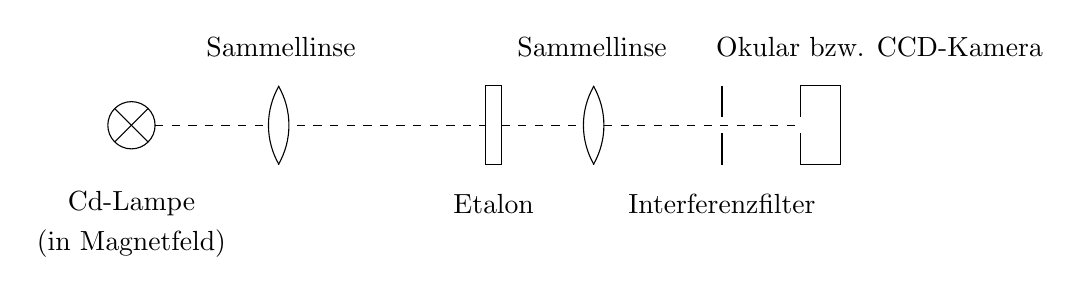
\begin{tikzpicture}
    \draw (-1.5+2,0) circle (0.3);
    \draw (-0.21-1.5+2,-0.21) -- (0.21-1.5+2,0.21);
    \draw (-0.21-1.5+2,0.21) -- (0.21-1.5+2,-0.21);
    \draw (5,-0.5)--(5,0.5)--(5.2,0.5)--(5.2,-0.5)--(5,-0.5);
    \draw (1.5+1,0) arc (0:30:1);
    \draw (1.5+1,0) arc (0:-30:1);
    \draw (1.24+1,0) arc (180:150:1);
    \draw (1.24+1,0) arc (180:210:1);
    \draw (6.5,0) arc (0:30:1);
    \draw (6.5,0) arc (0:-30:1);
    \draw (6.24,0) arc (180:150:1);
    \draw (6.24,0) arc (180:210:1);
    \draw (8,-0.5)--(8,-0.1);
    \draw (8,0.5)--(8,0.1);
    \draw (9,-0.1)--(9,-0.5)--(9.5,-0.5)--(9.5,0.5)--(9,0.5)--(9,0.1);
    \draw [dashed] (0.8,0)--(2.2,0);
    \draw [dashed] (2.6,0)--(5,0);
    \draw [dashed] (5.2,0)--(6.2,0);
    \draw [dashed] (6.5,0)--(9,0);
    \draw (0.5,-1) node {Cd-Lampe};
    \draw (0.5,-1.5) node {(in Magnetfeld)};
    \draw (2.4,1) node {Sammellinse};
    \draw (5.1,-1) node {Etalon};
    \draw (6.35,1) node {Sammellinse};
    \draw (8,-1) node {Interferenzfilter};
    \draw (10,1) node {Okular bzw. CCD-Kamera};
  \end{tikzpicture}
  \caption{Aufbau zum Zeemann-Effekt (nicht maßstabsgetreu)}
  \label{fig:aufbau}
\end{figure}
